\documentclass{article}
\usepackage{graphicx}
\graphicspath{{images/}}
\begin{document}
% .aux file is needed for image labelling.
% Images can be captioned, labelled and referenced by means of the figure environment.
\begin{figure}[h]
    \centering
    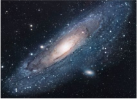
\includegraphics{universe}
    \caption{A nice plot.}
    \label{fig:1}
\end{figure} 

% Twice compilation is needed for getting the .aux file and correcting references respectively.
As you can see in figure \ref{fig:1}, the function grows near the origin. This example is on page \pageref{fig:1}.

\end{document}